%Todo
%Bibliography

%Table?
%Colors

%For TikZ
%latex figure.tex
%dvisvgm figure.dvi

%Examples of url links
%TexML

%Some documentation/readme
%author seems not to being passed to the epub.
%XY-Pic/TikZ: cannot be done inline at the moment


\documentclass[12pt,reqno]{amsbook}


%% \usepackage[english]{babel}  %Language needs to be specified for accessibility; currently this is not working well with latexml

% Math
\usepackage{amsmath, amssymb, amsthm}

%Graphics
\usepackage{graphicx}

% Bibliography
%\usepackage[backend=biber,style=numeric,maxbibnames=99]{biblatex}
%\addbibresource{thesis.bib}

% Layout
\usepackage{geometry}
\geometry{margin=1in}

% Theorem environments
\newtheorem{theorem}{Theorem}[chapter]
\newtheorem{lemma}[theorem]{Lemma}
\theoremstyle{definition}
\newtheorem{definition}[theorem]{Definition}

% Hyperref
\usepackage[pdfusetitle]{hyperref}

\begin{document}

% Title metadata

\newcommand{\thetitle}{A Sample Thesis in Mathematics}
\title{\thetitle}
\date{\today}
\newcommand{\institution}{University of Illinois Chicago} 
\newcommand{\degree}{Doctor of Philosophy}
\newcommand{\advisor}{Prof.~Ada Lovelace}
\newcommand{\theauthor}{A.~Student}
\author{\theauthor}

\frontmatter

% Custom title page
\begin{titlepage}
    \centering
    {\Large \institution\par}
    \vspace{2cm}
    {\Large \thetitle \par}
    \vspace{2cm}
    {\Large by\par}
    \vspace{0.5cm}
    {\Large \theauthor\par}
    \vfill
    A thesis submitted in partial fulfillment of the requirements \\
    for the degree of  \degree \\
    \vspace{0.5cm}
    Advisor: \advisor \\
    \vspace{1cm}
    \makeatletter\@date \makeatother
\end{titlepage}

\begin{abstract}
This thesis investigates XYZ. We show results about ...
\end{abstract}

\tableofcontents

\mainmatter

\chapter{Introduction}
This is the introduction chapter. We cite some classic works \cite{einstein,serre}.

% jpg, jpeg
% Test SVG
\section{Motivation}
\begin{figure}\label{fig1}
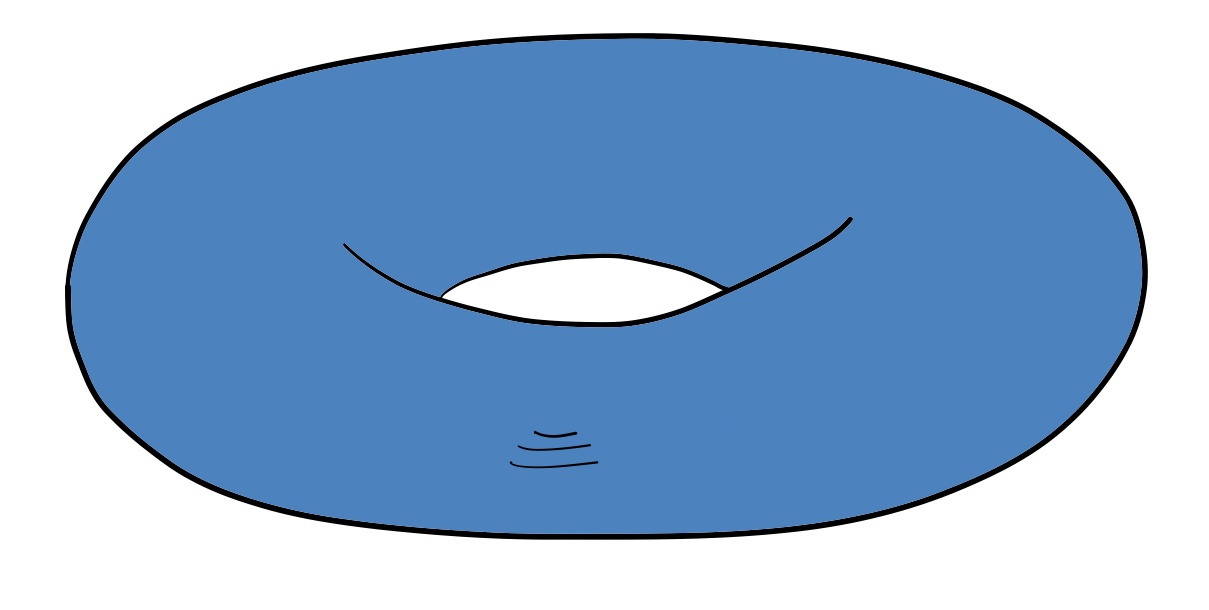
\includegraphics[alt="Description of Image that serves the same purpose",scale=0.3]{torus.jpg}
\caption{This is a torus jpg}
\end{figure}

%% PDF images do not work
%\begin{figure}\label{fig1}
%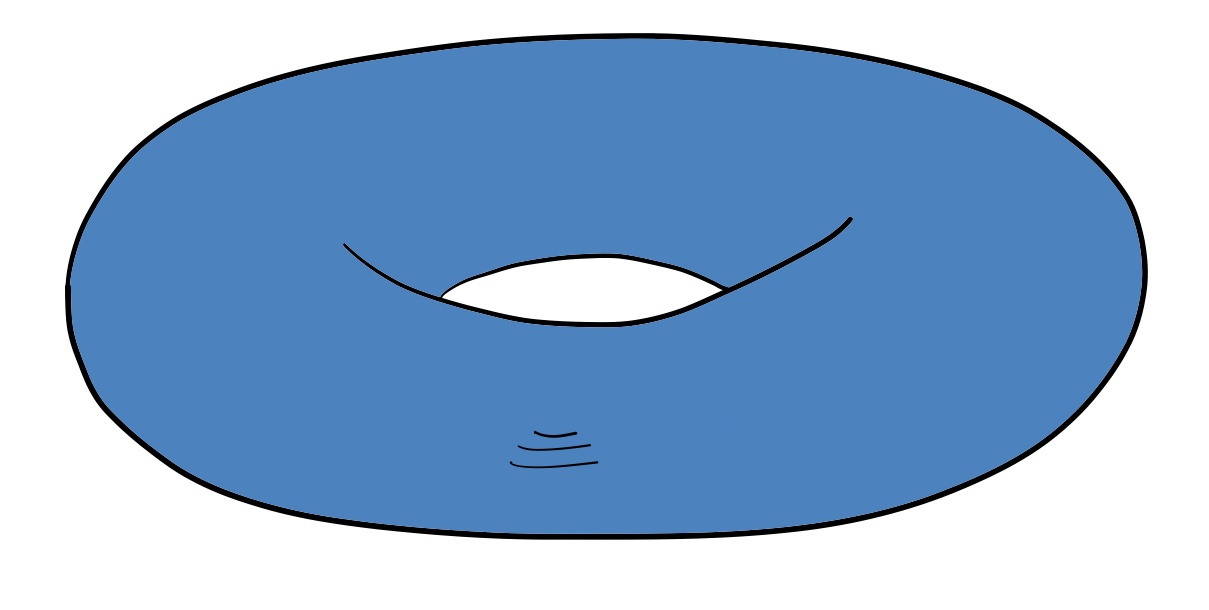
\includegraphics[alt="Description of Image that serves the same purpose",scale=0.3]{torus.pdf}
%\caption{This is a torus pdf}
%\end{figure}

\subsection{Historical context}
A brief overview of how the problem developed.
\begin{equation}\label{eq1}\int_0^1 f(x) dx = 2\end{equation}
How to solve \eqref{eq1}
\subsection{Open questions}
Some questions remain open for future work.

\section{Outline of the thesis}
We summarize the structure of the thesis.

\chapter{Background}
This chapter gives necessary background.

\section{Group theory}
\begin{definition}
A group is a set $G$ with a binary operation satisfying closure, associativity, identity, and inverses.
\end{definition}

\begin{theorem}
Every finite subgroup of the multiplicative group of a field is cyclic.
\end{theorem}

\begin{proof}
This is a standard result from algebra.
\end{proof}

\section{Linear representations}
As explained in Serre's book \cite{serre}, representation theory plays a key role.

\chapter{Main Results}
Here we present the main contributions of the thesis.

\section{First main result}
Statement and proof go here.

\section{Second main result}
Another significant theorem.

\appendix
\chapter{Technical Lemmas}
Here we collect some supporting lemmas.

%\backmatter


\end{document}
